\documentclass{article}
\usepackage{graphicx}

\begin{document}

\title{Introduction to \LaTeX{}}
\author{Jordan Hong}

\maketitle

\begin{abstract}
    This is a tester file for latex compiling.
\end{abstract}

\section{Introduction}
Here is the text of your introduction.

\begin{equation}
    \label{simple_equation}
    \alpha = \sqrt{ \beta }
\end{equation}

\subsection{Subsection Heading Here}


        Lorem ipsum dolor sit amet, consectetur adipiscing elit. Vestibulum neque metus, fermentum eget rutrum eget, finibus nec eros. Cras luctus et erat tincidunt ornare. Aliquam fermentum neque elit, ut finibus ligula ornare id. Duis libero lectus, molestie tristique turpis quis, condimentum gravida neque. Vestibulum tempus, arcu ut semper mattis, sem justo blandit erat, in maximus nulla libero non tortor. Donec non urna ut lacus pharetra facilisis. Donec mattis enim at sapien lacinia dictum. Suspendisse commodo vitae nibh ut accumsan. Sed elementum lectus diam, eget blandit turpis convallis vitae. Quisque vitae ligula justo. Suspendisse sit amet mi est. Nulla facilisi. Vivamus leo odio, ullamcorper a tortor vel, convallis ullamcorper velit. Nunc condimentum nibh ligula. Etiam porta massa a diam pulvinar vestibulum.

        Praesent laoreet ipsum vitae purus ullamcorper, sed lacinia neque euismod. Aliquam iaculis faucibus mauris rhoncus elementum. Nunc vitae euismod urna, a finibus ex. Fusce tempus neque sit amet elit commodo, non ullamcorper sapien lacinia. Phasellus molestie risus vel porttitor maximus. Proin non purus in arcu malesuada imperdiet. Nam id lacus quis ante tempus varius. Mauris ut nisi felis. Nam in volutpat urna. Integer maximus, dolor eget congue imperdiet, quam mauris sodales massa, nec egestas dui elit ut elit. Etiam volutpat lorem a ligula cursus, et dictum nunc ullamcorper. Morbi nunc risus, iaculis id lectus non, feugiat scelerisque orci. Proin euismod ullamcorper diam. Mauris et arcu sed velit rhoncus maximus.

        Fusce vel leo leo. Interdum et malesuada fames ac ante ipsum primis in faucibus. Morbi sit amet congue neque, quis luctus est. Donec in porta elit, eget pulvinar odio. Interdum et malesuada fames ac ante ipsum primis in faucibus. Nunc sollicitudin nibh a velit pharetra ultrices. Maecenas dignissim libero vitae urna fringilla fringilla. Quisque sapien arcu, aliquam at facilisis quis, sagittis eget odio. Quisque nec dolor et lectus tempor accumsan at sit amet magna.

        Suspendisse efficitur, lectus a ultricies interdum, ex nisl dignissim tortor, vel dignissim lectus mi vitae nunc. Etiam nec lectus lacus. Ut semper bibendum orci, sed rhoncus eros sagittis eu. Quisque nec felis molestie, maximus mi non, vestibulum lorem. Proin justo purus, pellentesque ut viverra eu, cursus ut metus. Suspendisse est quam, venenatis quis sem at, dapibus luctus dolor. Suspendisse consequat porta tincidunt. 

\begin{figure}
    \centering
    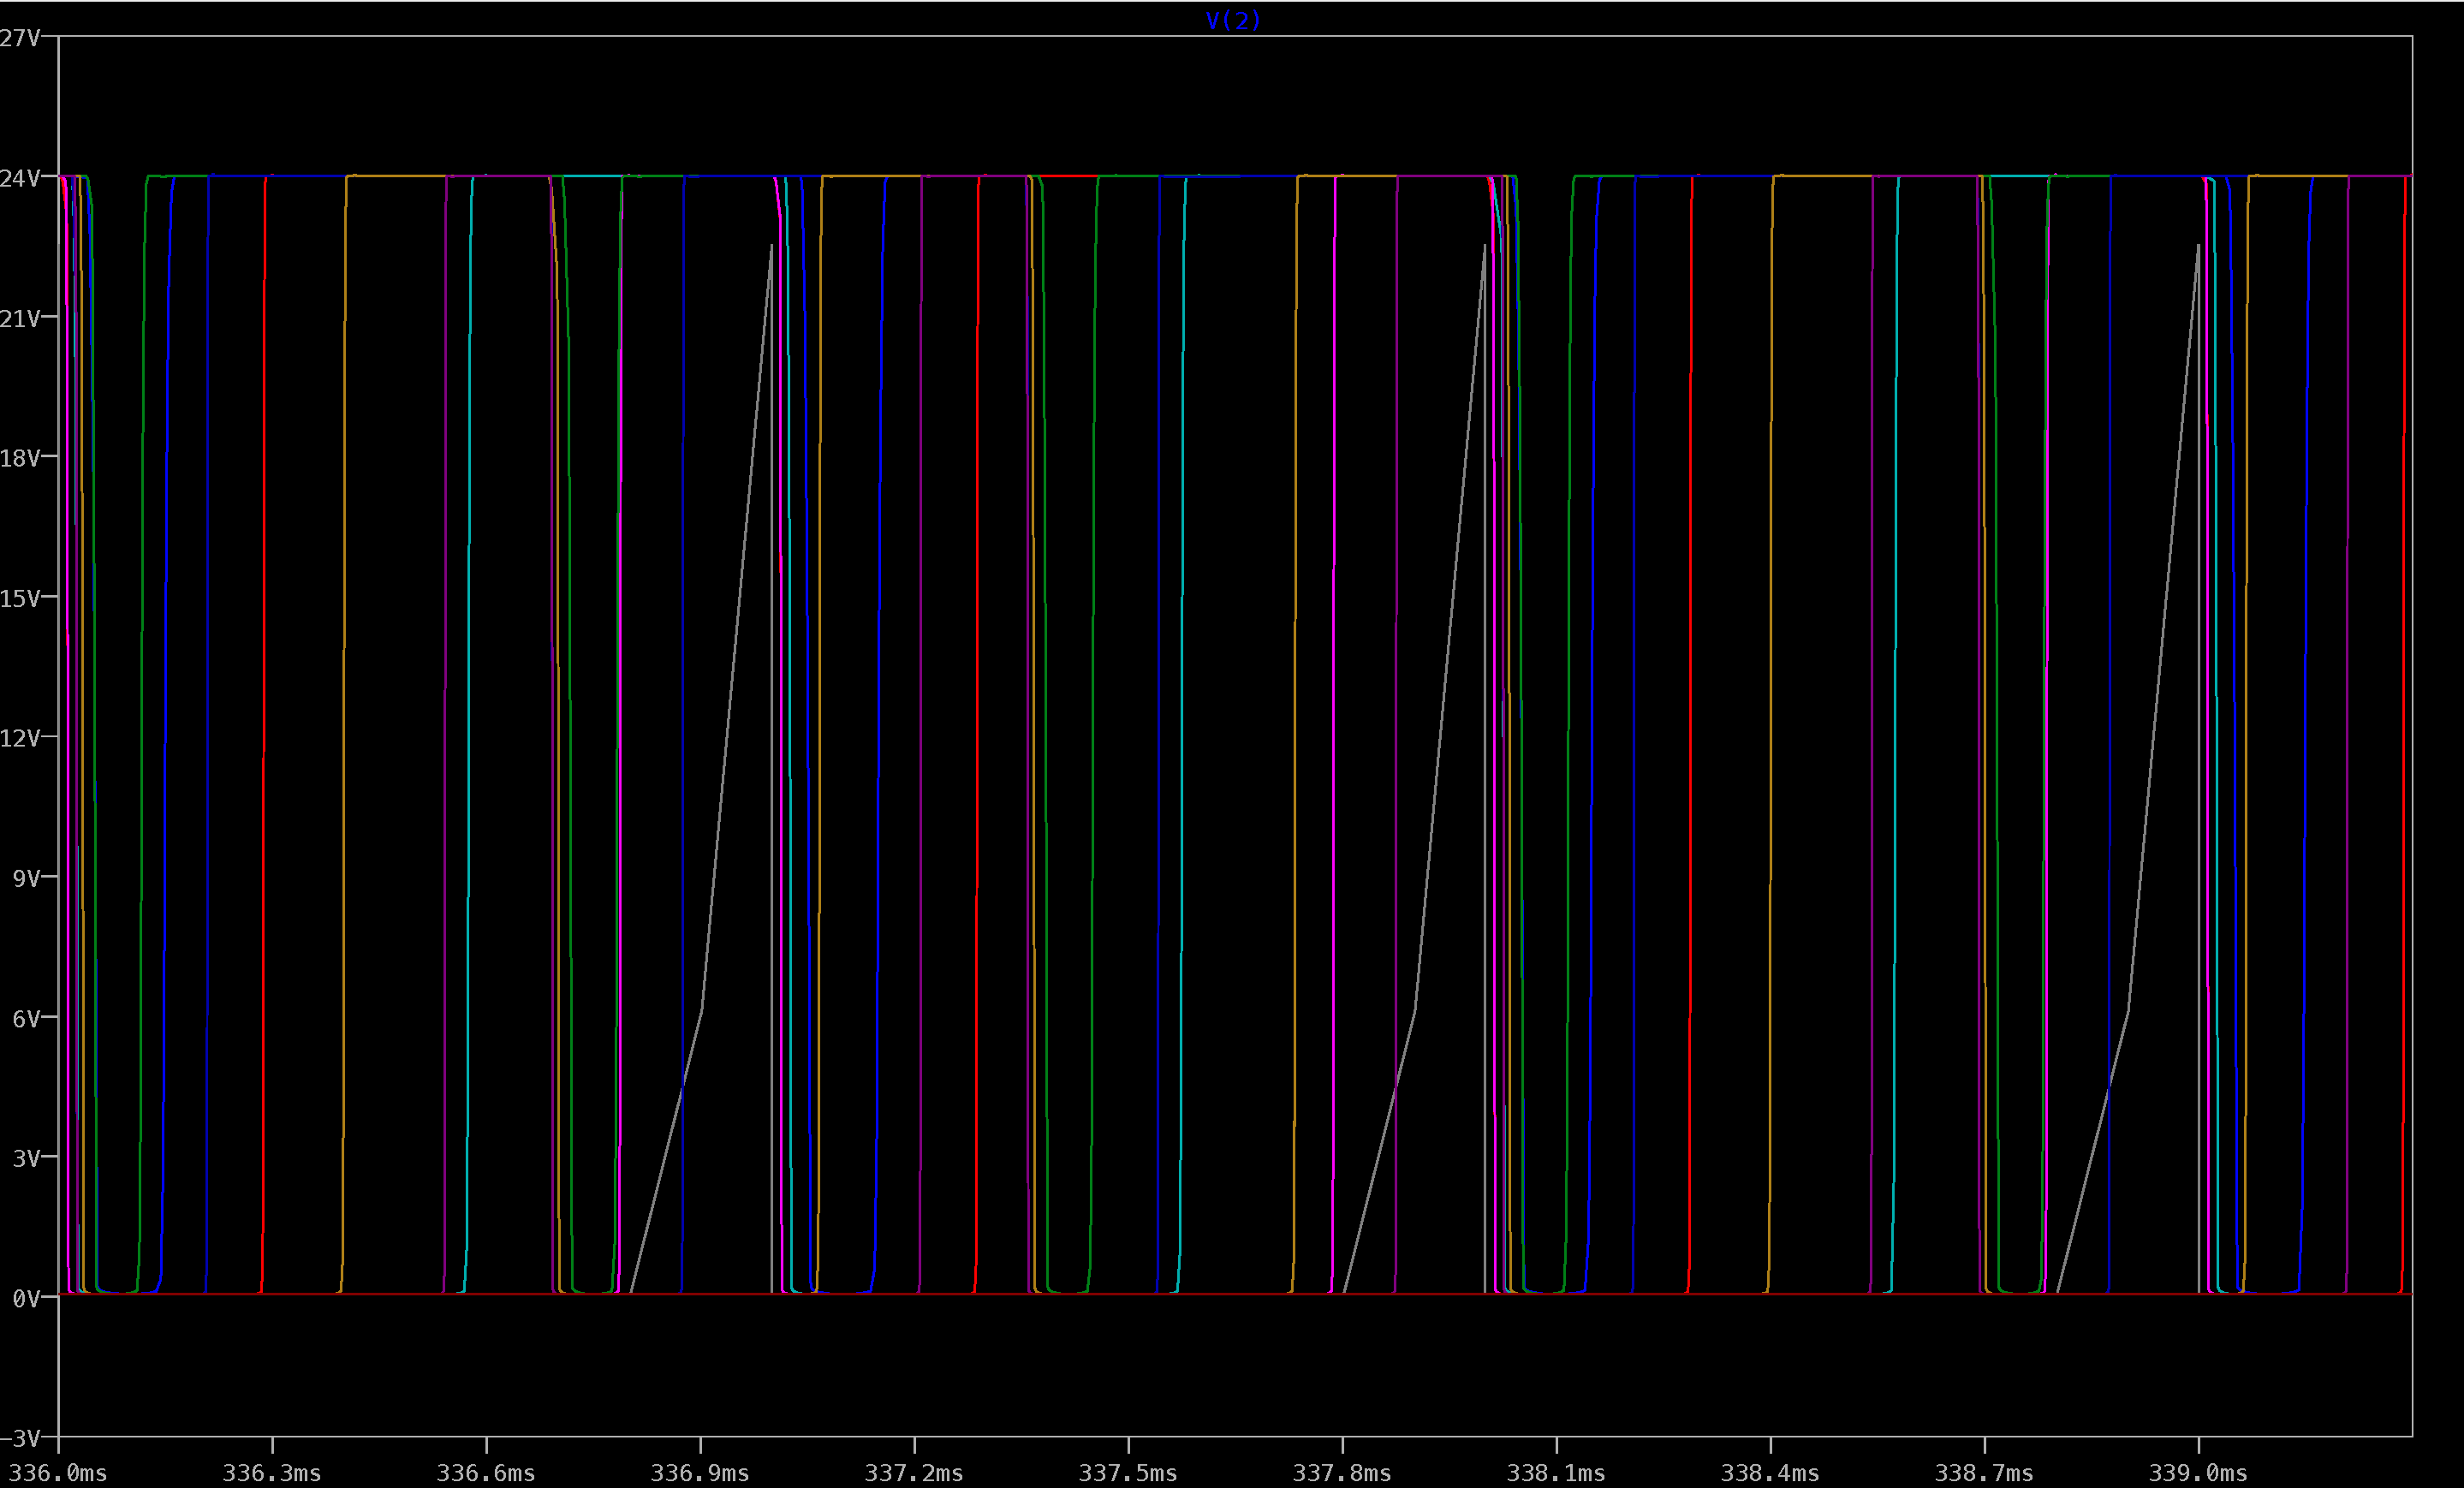
\includegraphics[width=3.0in]{my-simulation.png}
    \caption{Simulation Results}
    \label{simulationfigure}
\end{figure}

\section{Conclusion}
Write your conclusion here.

\end{document}
